\documentclass[11pt]{article}
\usepackage{graphicx}
\usepackage{subcaption}
\usepackage{wrapfig}
\title{Ubiquitous Genomics: Hackathon2}

\author{
  Maya Anand\\ mva2112@columbia.edu \and
  Anne Bozack\\ akb2134@cumc.columbia.edu \and
  Cheyenne Parsley\\ cep2141@columbia.edu \and
  Robert Piccone\\ rap2186@columbia.edu \and
  Daniel Speyer\\ dls2192@columbia.edu}
\begin{document}
\maketitle
\section*{Problem 1}
Number of 1D and 2D reads classified as failed: 265\\
Number of 1D and 2D reads classified as passed: 1082\\
Number of 2D reads classified as failed: 258\\
Number of 2D reads classified as passed: 1082\\
Fraction of 2D reads in failed folder: 0.97358490566\\
Fraction of 2D reads in passed folder: 1.0\\
\section*{Problem 2}
\begin{wrapfigure}{r}{2.5in}
  \vspace{-20pt}
  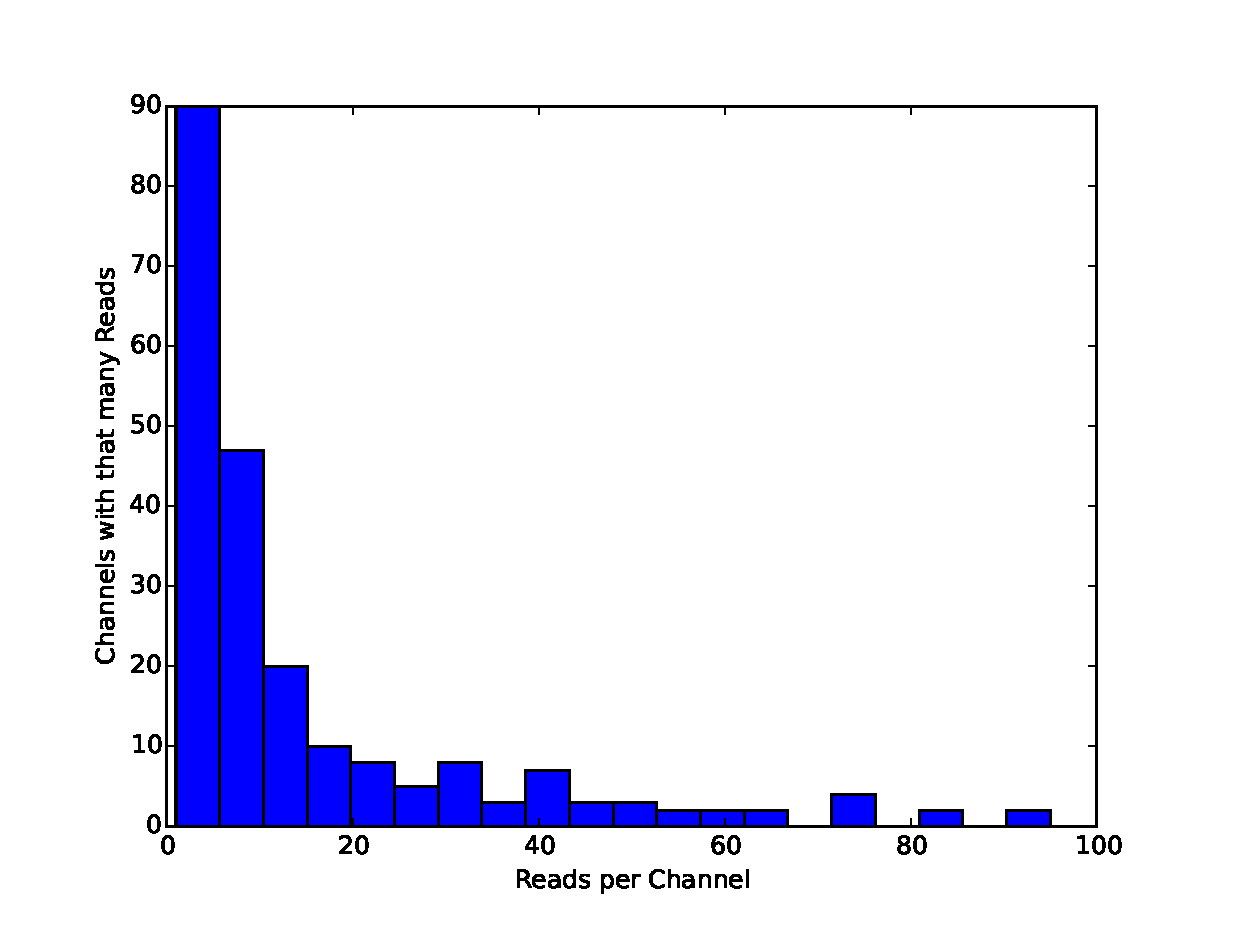
\includegraphics[width=2.5in]{part2hist}
  \vspace{-20pt}
\end{wrapfigure}
2 channels had at least one read, and 1 had at least five.  
This compares with 434 ``active'' channels during initialization, and 651 immediately after loading fuel

The average channel had 1262.0 reads. 
Channel 29 had 2520 reads, which was the most.

Just for fun, here's a histogram of reads per channel\\
\section*{Problem 3}
\begin{tabular}{cc}
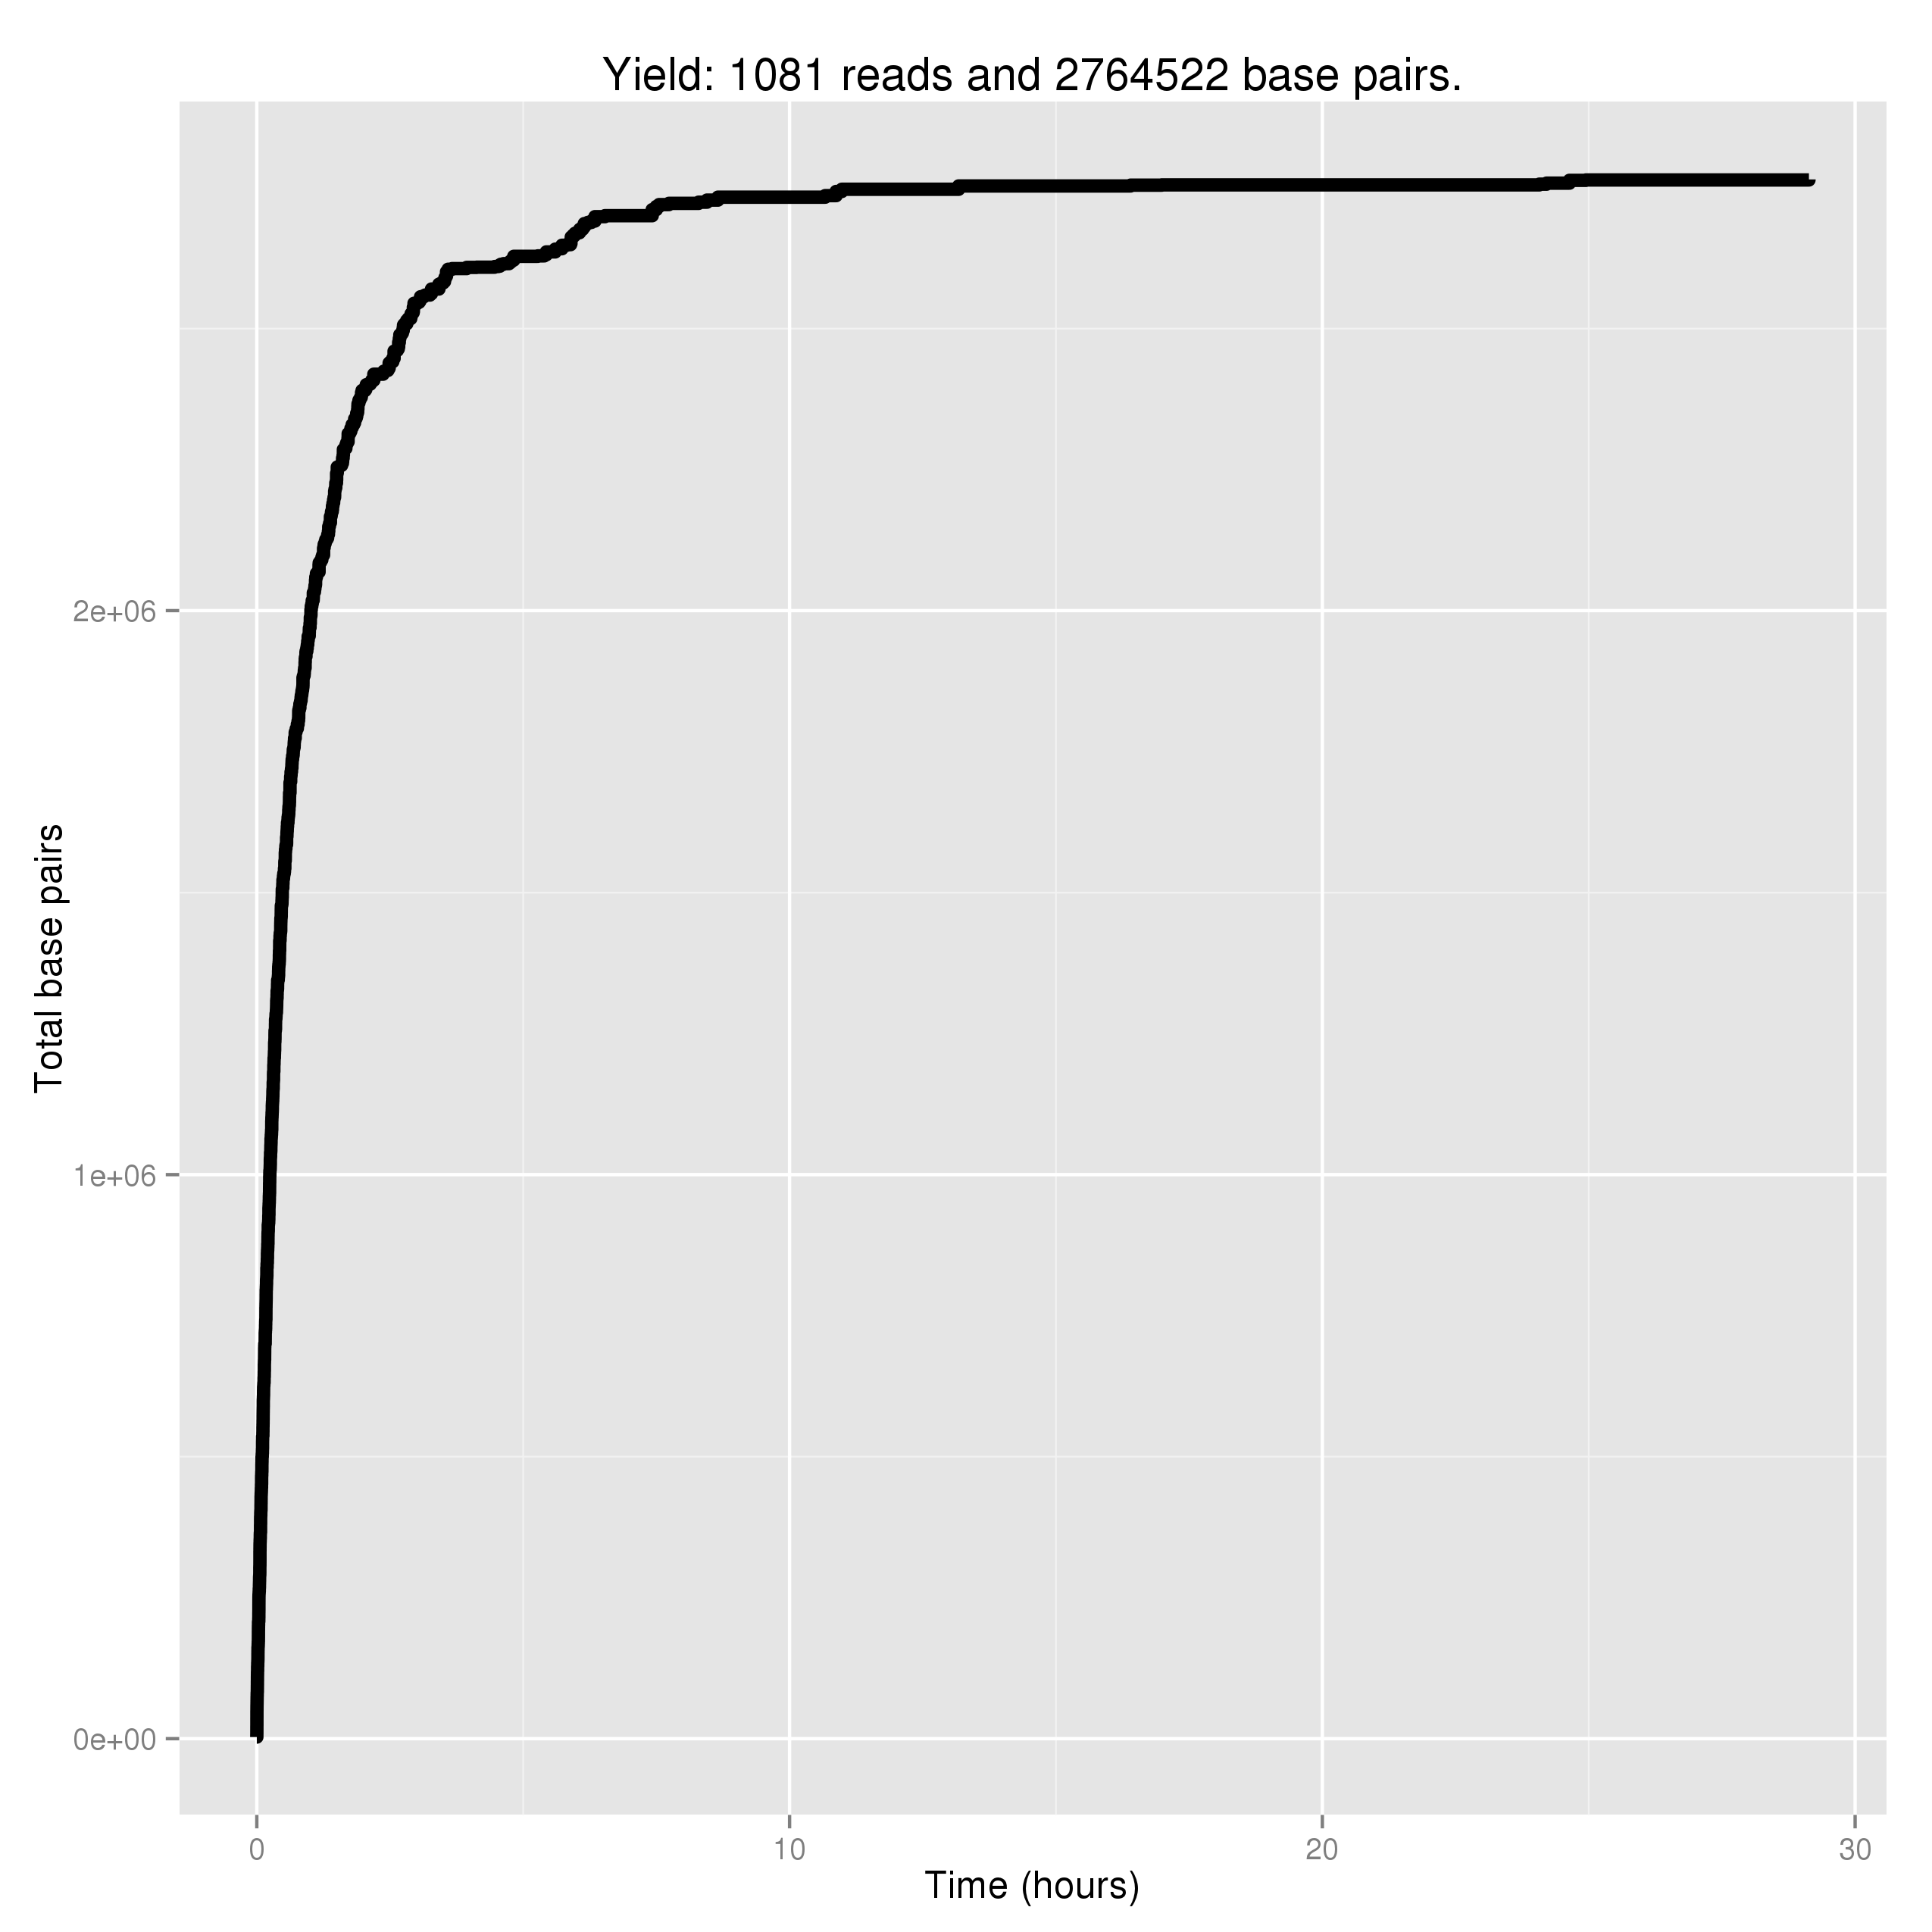
\includegraphics[width=.48\textwidth]{cumnucpass}
&
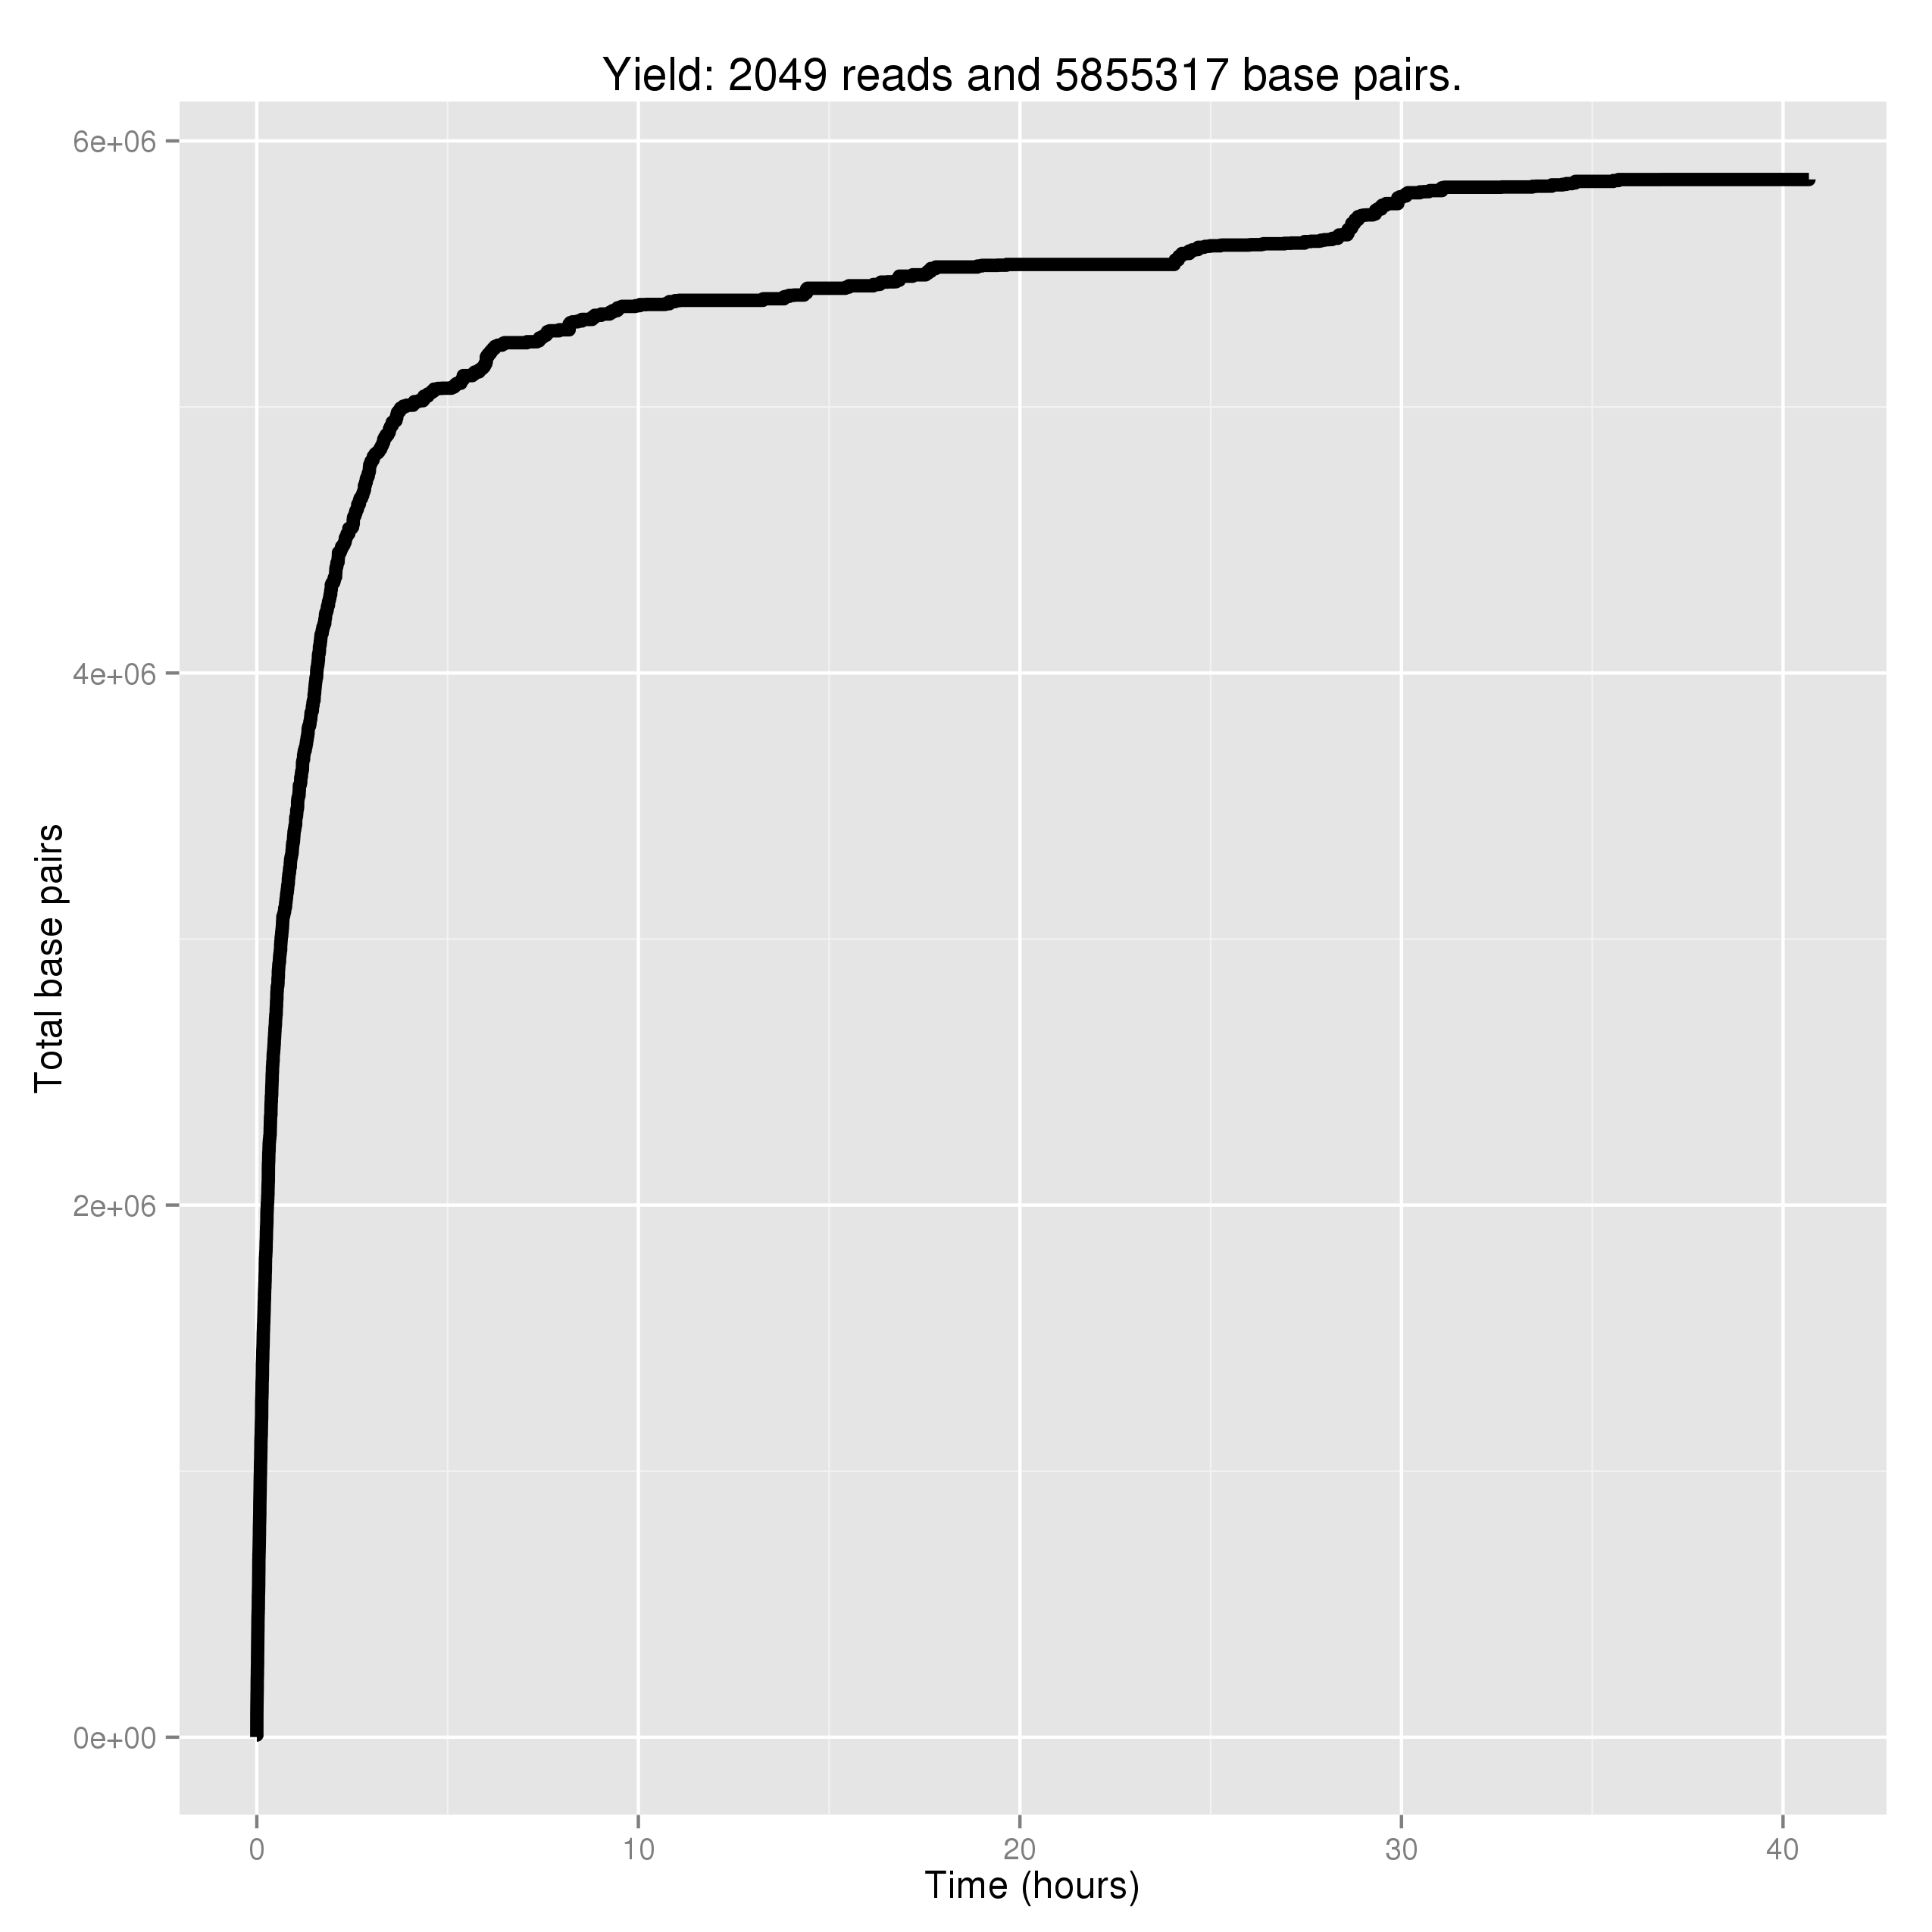
\includegraphics[width=.48\textwidth]{cumnucfail}
\\
Passed Reads
&
Failed Reads
\end{tabular}
\section*{Problem 4}
\subsection*{1D reads}

        The following histograms show the length distribution of 1D reads (both template and complement) for passes and fails.

        \begin{tabular}{cc}
          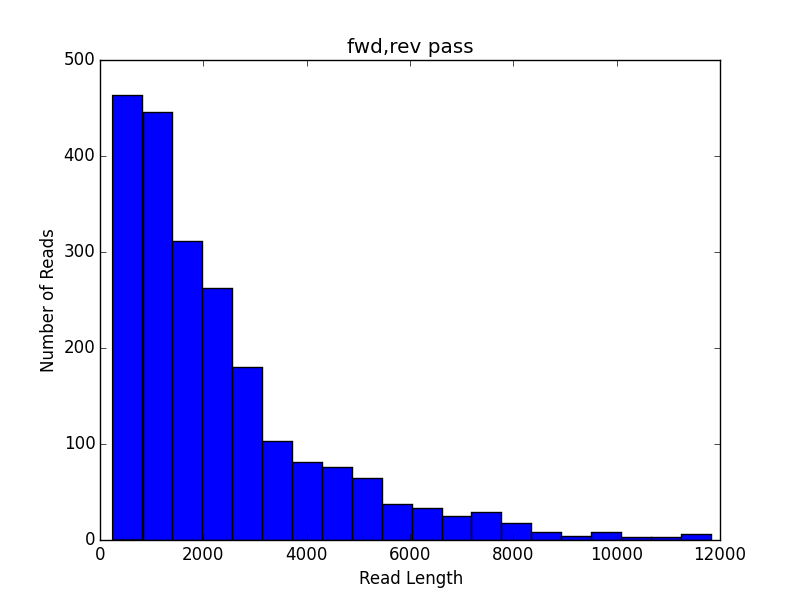
\includegraphics[width=.48\textwidth]{1Dpasses}
          &
          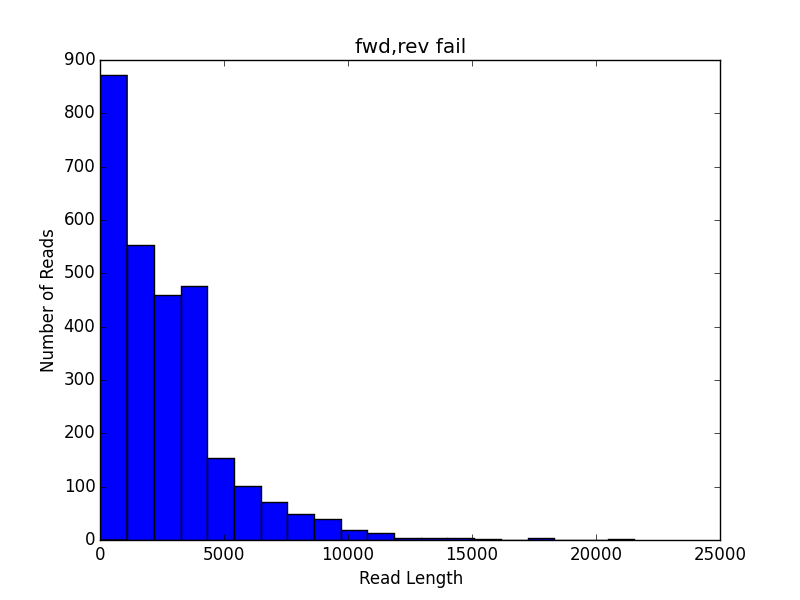
\includegraphics[width=.48\textwidth]{1Dfailures}
          \\
          Passed Reads
          &
          Failed Reads
        \end{tabular}
        

\subsection*{2D reads}

        The following histograms show the length distribution of 2D reads for passes and fails.

        
        \begin{tabular}{cc}
          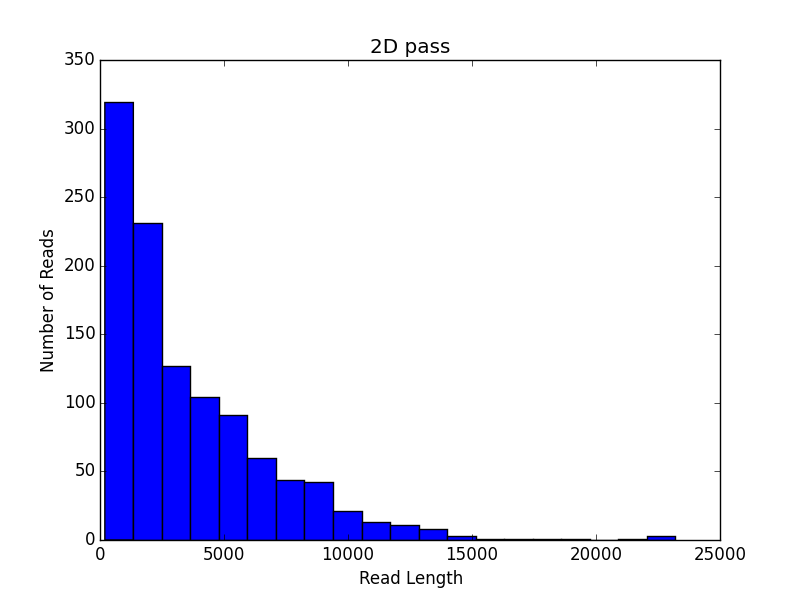
\includegraphics[width=.48\textwidth]{2Dpasses}
          &
          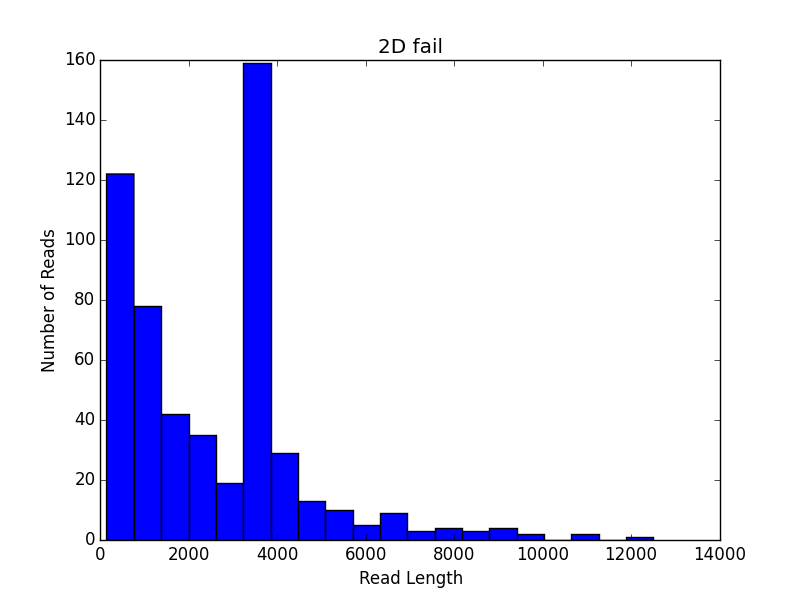
\includegraphics[width=.48\textwidth]{2Dfailures}
          \\
          Passed Reads
          &
          Failed Reads
        \end{tabular}

        
\subsection*{1D and 2D reads}

        The following histogramss show the cumulative length distribution of both 1D and 2D reads for passes and fails.

        
        \begin{tabular}{cc}
          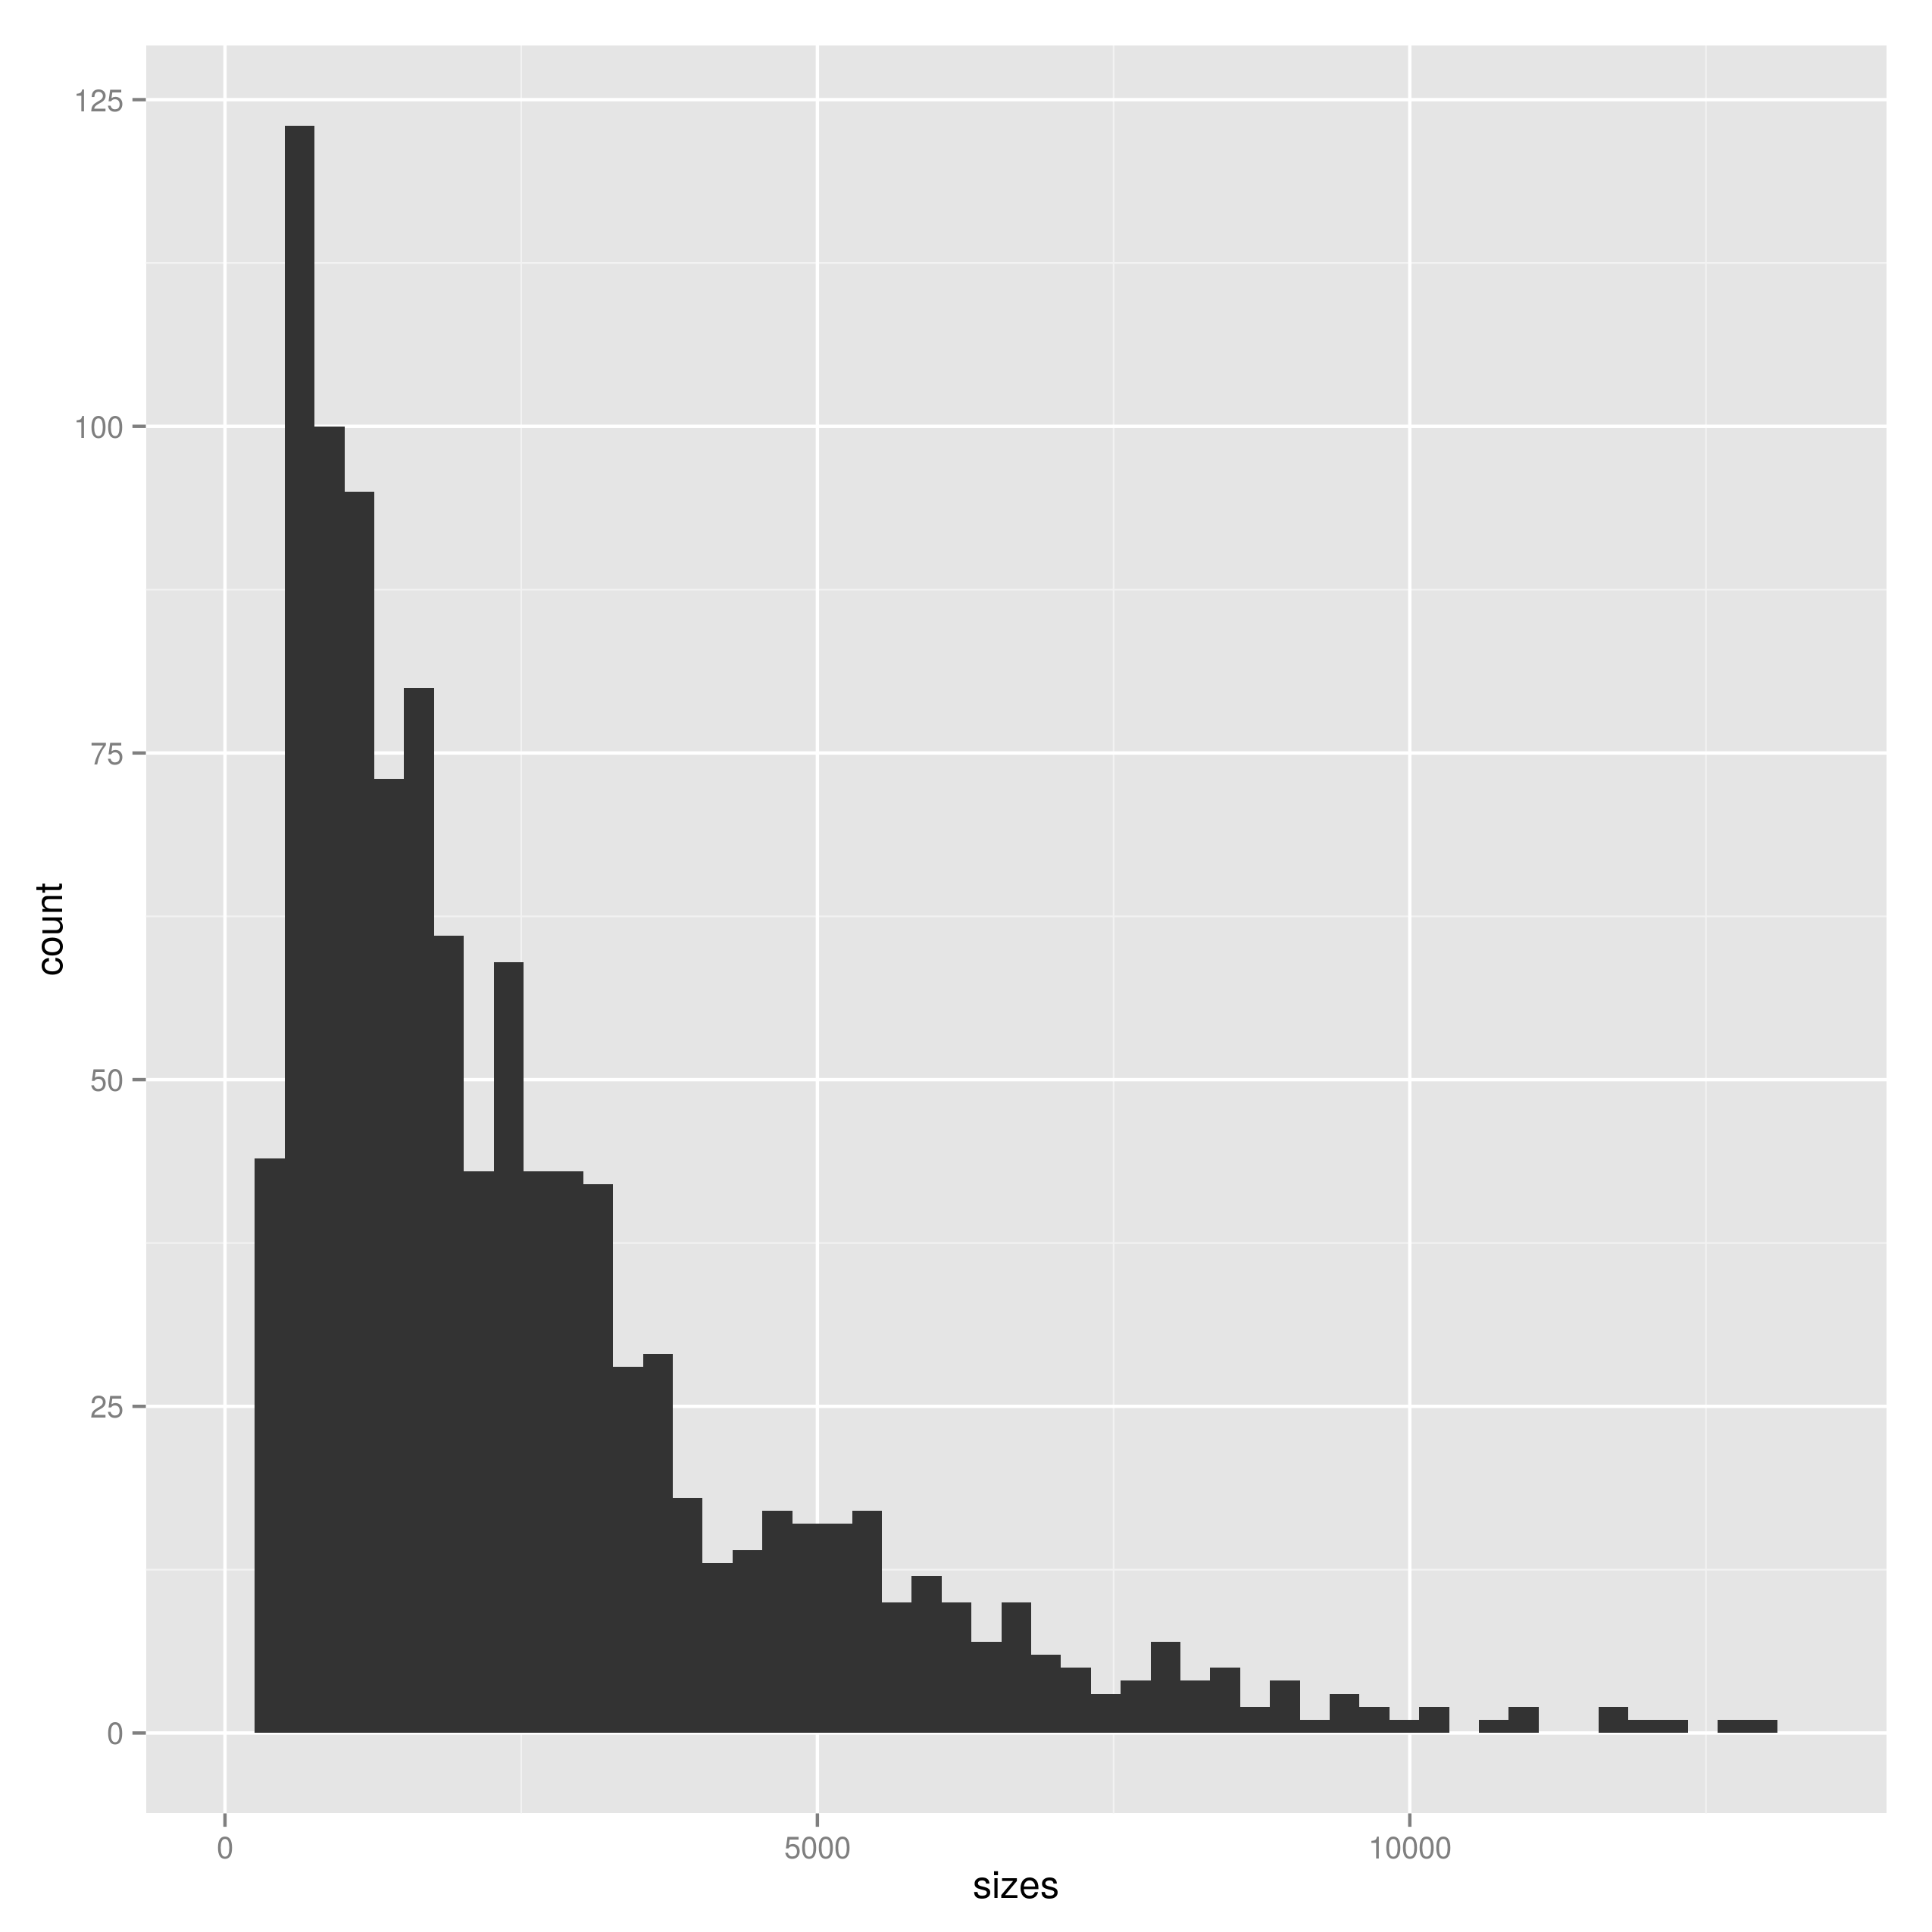
\includegraphics[width=.48\textwidth]{histallpass}
          &
          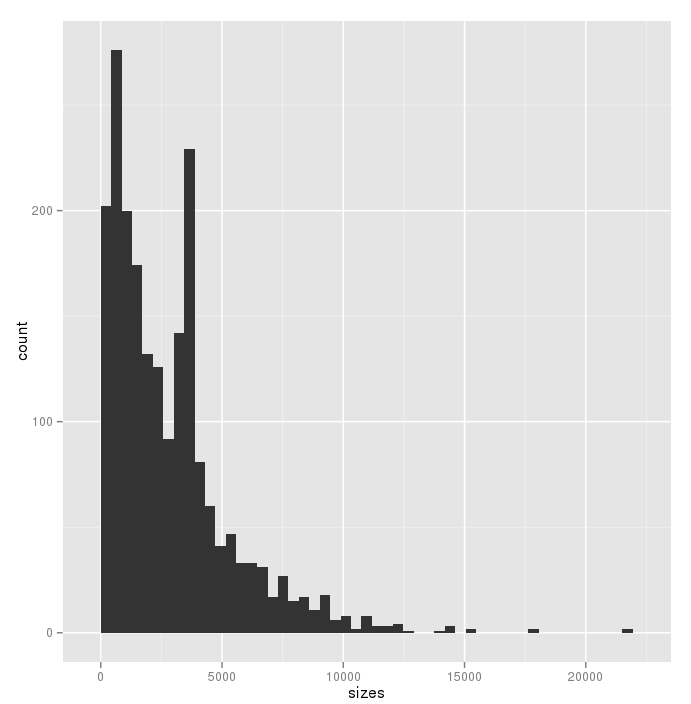
\includegraphics[width=.48\textwidth]{histallfail}
          \\
          Passed Reads
          &
          Failed Reads
        \end{tabular}
\section*{Problem 5}

LONGEST TEMPLATE READ\\
From file: .\\
Number of nucleotides: 5\\

LONGEST COMPLEMENT READ\\
From file: .\\
Number of nucleotides: 5\\

LONGEST 2D READ\\
From file: MINION02\_Hackathon2\_group4\_TeamAWESOME\_4029\_1\_ch9\_file8\_strand.fast5\\
Number of nucleotides: 23196\\
\end{document}
